\subsection{Matriz PEYEA}

La matriz PEYEA (matriz de la posición estratégica y la evaluación de la acción) nos permite determinar estrategias apropiadas para la organizacion y determinar si estas son agresivas, conservadoras, defensivas o competitivas. Alli se representan dos dimensiones internas (fuerzas financieras y ventajas competetitivas) y dos dimensiones externas(estabilidad del ambiente y fuerza de la industria) 

Los pasos necesarios para elaborar una matriz PEYEA son:

1. Seleccionar variables para definir fortalezas financieras, ventaja competetitiva, estabilidad ambiental y fortaleza industrial.

2. Asignar un valor numerico a cada una de las variables que integran las dimensiones de FF y FI, siendo +1 como peor y +6 como mejor

3. Asignar un valor numerico a cada una de las variables que integran las dimensiones de EA y VC, siendo +1 como mejor y +6 como peor.

4. Calcular un puntaje promedio para cada una de las dimensiones, sumando los valores asignados a las variables y dividiéndolo por el total de ellas.

5. 



\begin{enumerate}
    \item Seleccionar una serie de variables para definir las fortalezas financieras, la ventaja competitiva, la estabilidad ambiental y la fortaleza industrial.
    
    \item Asignar un valor numérico a cada una de las variables que integran las dimensiones FF y FI, siendo +1 como peor y +6 como mejor. Además, asignar a cada variable que integra la dimensión EA y VC los valores -1 como mejor y -6 como peor.
    
    \item Calcular un puntaje promedio para cada una de las dimensiones, sumando los valores asignados a las variables y dividiéndolo por el total de ellas.
    
    \item Registrar los puntajes promedio de las dimensiones correspondientes a la matriz PEYEA.
    
    \item Sumar los dos puntajes del eje x y registrar el punto resultante en X. Sumas los dos puntos del eje y y registrar el punto resultante en Y. Registra la intersección del nuevo punto xy.
    
    \item Dibujar un vector direccional desde el origen de la matriz PEYEA que pase por el nuevo punto de intersección. Este vector revela el tipo de estrategia recomendada: participación relativa en el mercado, competitiva, defensiva o conservadora.
\end{enumerate}

La matriz PEYEA que se ha obtenido es la siguiente:

\vspace{2mm}
\begin{minipage}{0.9\textwidth}
\centering
\captionof{table}[{Matriz PEYEA.}]{ Matriz PEYEA }
\label{peyea}
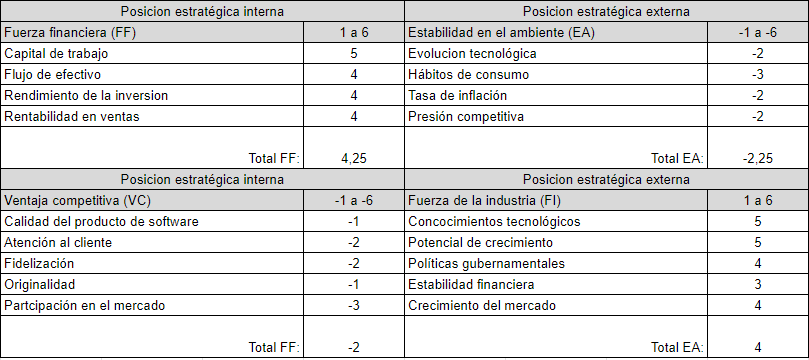
\includegraphics[width=1\textwidth]{Images/tablaPEYEA.png}
\fnote{Nota. \textup{Fuente : Autores.}}
\end{minipage}

Donde, el valor de X es el resultado del balance entre la Fuerza Financiera (FF) y la estabilidad del ambiente (EA) y el valor de Y es el resultado del balance entre la Ventaja Competitiva (VC) y la fortaleza industrial (FI).

\vspace{1mm}
\begin{minipage}{\textwidth}
\centering
\captionof{table}[{Matriz PEYEA, Valor X.}]{ Matriz PEYEA, Valor X }
\label{peyeax}
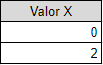
\includegraphics[\textwidth]{Images/valorX.png}
\fnote{Nota. \textup{Fuente : Autores.}}
\end{minipage}

\vspace{1mm}
\begin{minipage}{\textwidth}
\centering
\captionof{table}[{Matriz PEYEA, Valor Y.}]{ Matriz PEYEA, Valor Y }
\label{peyeay}
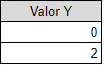
\includegraphics[\textwidth]{Images/valorY.png}
\fnote{Nota. \textup{Fuente : Autores.}}
\end{minipage}

Representados gráficamente en la siguiente imagen:

\vspace{2mm}
\begin{minipage}{0.9\textwidth}
\centering
\captionof{figure}[{Representación gráfica Matriz PEYEA.}]{ Representación gráfica Matriz PEYEA }
\label{peyeagrafico}
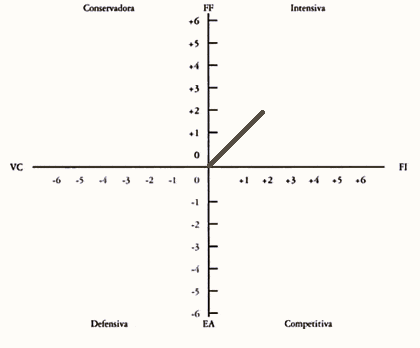
\includegraphics[width=0.6\textwidth]{Images/PEYEA.png}
\fnote{Nota. \textup{Fuente : Autores.}}
\end{minipage}

Como conclusión, la empresa HIRE.IT SAS se encuentra posicionada dentro del primer cuadrante, lo cual significa que está en el cuadrante intensivo, lo que permite utilizar sus fortalezas internas para lograr un adecuado uso de las oportunidades externas que se presentan, evitando las amenazas del entorno y las debilidades que posee.